\documentclass[aspectratio=169]{beamer}
\makeatletter
\def\input@path{{../common/}{../guide/}{../data/}{../code/}}
\makeatother
\usetheme{Bruno}
\usepackage{amsmath}
\usepackage{amssymb}
\usepackage{siunitx}
\usepackage{float}
\usepackage{tikz}
\def\checkmark{\tikz\fill[scale=0.4](0,.35) -- (.25,0) -- (1,.7) -- (.25,.15) -- cycle;} 
\usepackage{url}
\usepackage[siunitx,american,RPvoltages]{circuitikz}
\ctikzset{capacitors/scale=0.7}
\ctikzset{diodes/scale=0.7}
\usepackage{tabularx}
\newcolumntype{C}{>{\centering\arraybackslash}X}
\renewcommand\tabularxcolumn[1]{m{#1}}% for vertical centering text in X column
\usepackage{tabu}
\usepackage[spanish,es-tabla,activeacute]{babel}
\usepackage{babelbib}
\usepackage{booktabs}
\usepackage{pgfplots}
\usepackage{hyperref}
\hypersetup{colorlinks = true,
            linkcolor = black,
            urlcolor  = blue,
            citecolor = blue,
            anchorcolor = blue}
\usepgfplotslibrary{units, fillbetween} 
\pgfplotsset{compat=1.16}
\usepackage{bm}
\usetikzlibrary{arrows, arrows.meta, shapes, 3d, perspective, positioning,mindmap,trees,backgrounds}
\renewcommand{\sin}{\sen} %change from sin to sen
\usepackage{bohr}
\setbohr{distribution-method = quantum,insert-missing = true}
\usepackage{elements}
\usepackage{verbatim}
\usepackage[edges]{forest}
\usepackage{etoolbox}
\usepackage{schemata}
\usepackage{appendix}
\usepackage{listings}

\definecolor{color_mate}{RGB}{255,255,128}
\definecolor{color_plas}{RGB}{255,128,255}
\definecolor{color_text}{RGB}{128,255,255}
\definecolor{color_petr}{RGB}{255,192,192}
\definecolor{color_made}{RGB}{192,255,192}
\definecolor{color_meta}{RGB}{192,192,255}
\newcommand\diagram[2]{\schema{\schemabox{#1}}{\schemabox{#2}}}

\definecolor{codegreen}{rgb}{0,0.6,0}
\definecolor{codegray}{rgb}{0.5,0.5,0.5}
\definecolor{codepurple}{rgb}{0.58,0,0.82}
\definecolor{backcolour}{rgb}{0.95,0.95,0.92}

\lstdefinestyle{mystyle}{
    backgroundcolor=\color{backcolour},   
    commentstyle=\color{codegreen},
    keywordstyle=\color{magenta},
    numberstyle=\tiny\color{codegray},
    stringstyle=\color{codepurple},
    basicstyle=\ttfamily\footnotesize,
    breakatwhitespace=false,         
    breaklines=true,                 
    captionpos=b,                    
    keepspaces=true,                 
    numbers=left,                    
    numbersep=5pt,                  
    showspaces=false,                
    showstringspaces=false,
    showtabs=false,                  
    tabsize=2
}

\lstset{style=mystyle}
\usepackage{unicode-math}
\setsansfont{Fira Sans}
\setmainfont{Fira Sans}
\setmathfont{Fira Math}

\title{Instrumentación I: \\ \emph{Transductores químicos}}
\author{
    Juan J. Rojas
}
\institute{Instituto Tecnológico de Costa Rica}
\date{\today}
\background{background.jpg}
\begin{document}
\sisetup{unit-math-rm=\mathrm,math-rm=\mathrm} % change sinitx font
\sisetup{output-decimal-marker = {,}}
\maketitle

% 8. Transductores químicos
% 8.1. Electroquímicos
% 8.2. Potenciométricos
% 8.3. Termoquímicos


\newcommand{\blackandwhite}{white} %change this at the end

\begin{frame}[t]{Unidades químicas}
    \begin{itemize}
        \item Mole (mol) = \si{6.02214e23} moleculas de la sustancia
        \item Masa molar (\si{g/mol})
        \item Partes por millón (ppm): \SI{1}{\milli\gram/\kilo\gram} u otra proporción análoga
        \item Partes por millón (ppm): \SI{1}{\micro\gram/\kilo\gram} u otra proporción análoga
    \end{itemize}
\end{frame}

\begin{frame}{Electroquímicos: oxidos metálicos}
    \begin{columns}[T, onlytextwidth]
        \begin{column}{0.55\textwidth}
            \begin{itemize}
                \item A temperaturas elevadas cambian su conductividad en presencia de gases
                \item Algunos oxidos que pueden usarse son de estaño (Sn0\textsubscript{2}), zinc (Zn0), 
                hierro (Fe\textsubscript{2}O\textsubscript{3}) y zirconio (ZrO\textsubscript{2}), entre otros
                \item La reacción con el gas a medir es de reducción
                \item Al bajar la concentración de gas reductor se reabsorbe oxigeno (oxidación)
                \item Algunos gases que se pueden medir son alchohol etílico, metano y monoxido de carbono
            \end{itemize}
        \end{column}
        \begin{column}{0.45\textwidth}
        \centering
        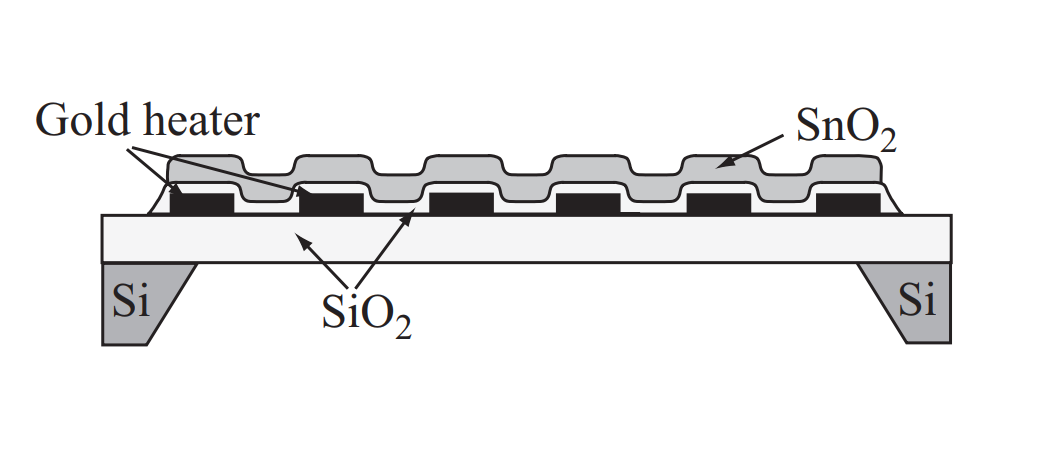
\includegraphics[width = \linewidth]{08_químicos/metal_oxido.png}
        \vspace*{1cm}
        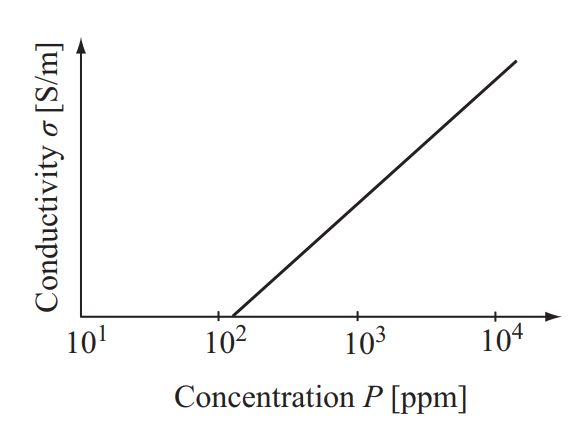
\includegraphics[width = 0.8\linewidth]{08_químicos/metal_oxido_sens.png}

        \tiny{Tomado de \cite{ida2013sensors}}
        \end{column}
    \end{columns}
\end{frame}

\begin{frame}{Electroquímicos: oxidos metálicos}
    \begin{columns}[T, onlytextwidth]
        \begin{column}{0.55\textwidth}
            La resistencia ($R$) del sensor se puede expresar como
            \begin{equation*} 
                R = aP^{-\alpha}
            \end{equation*}
            donde $a$ es una constante definida por el material y la construcción del sensor, 
            $P$ es la concentración del gas (ppm), y $\alpha$ es una constante relacionada al tipo de gas.
        \end{column}
        \begin{column}{0.45\textwidth}
        \centering
        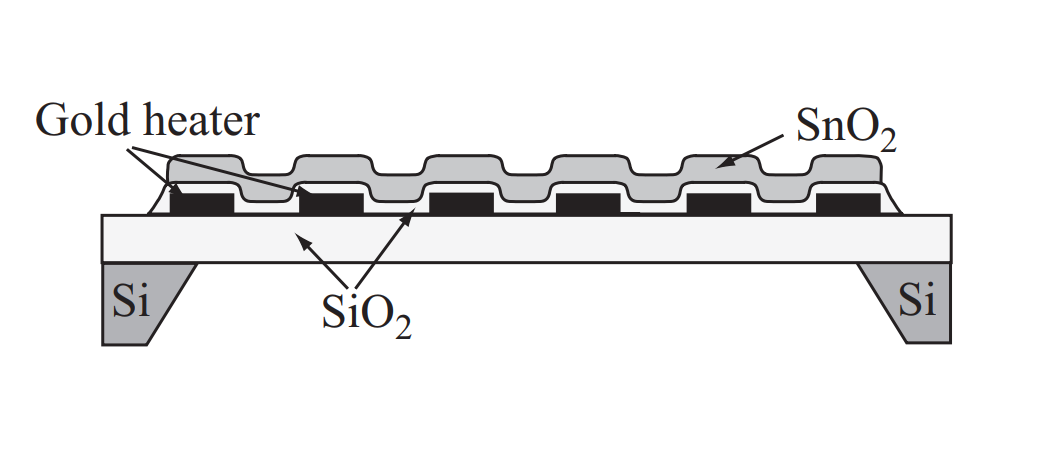
\includegraphics[width = \linewidth]{08_químicos/metal_oxido.png}
        \vspace*{1cm}
        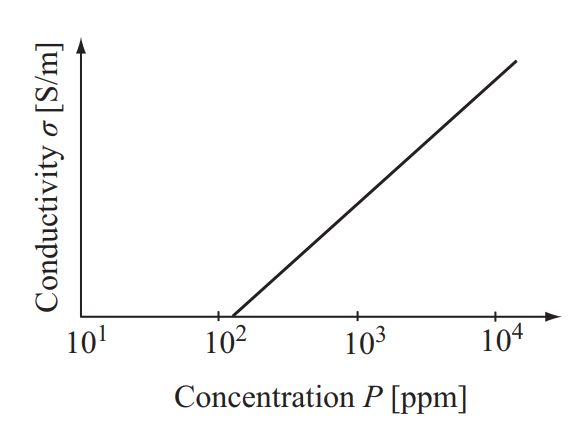
\includegraphics[width = 0.8\linewidth]{08_químicos/metal_oxido_sens.png}

        \tiny{Tomado de \cite{ida2013sensors}}
        \end{column}
    \end{columns}
\end{frame}

\begin{frame}{Electroquímicos: electrolito solido}
    \begin{columns}[T, onlytextwidth]
        \begin{column}{0.55\textwidth}
            \begin{itemize}
                \item Consiste en una celda galvánica, cuyos electrodos están en contacto
                con dos ambientes gaseosos a diferentes concentraciones
                \item El electrolito es un sólido cerámico que permite el paso de iones
                \item Los electrodos son metalicos, usualmente de platino
                \item Un ejemplo común es el sensor de oxígeno en gases de escape automotriz
            \end{itemize}
        \end{column}
        \begin{column}{0.45\textwidth}
        \centering
        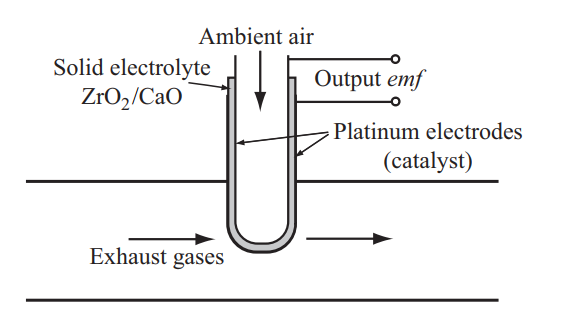
\includegraphics[width = \linewidth]{08_químicos/electrolito_solido_1.png}
        \vspace*{1cm}
        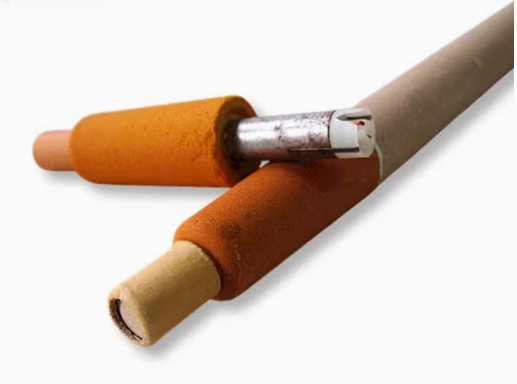
\includegraphics[width = 0.8\linewidth]{08_químicos/electrolito_solido_3.png}

        \tiny{Tomado de \cite{ida2013sensors}}
        \end{column}
    \end{columns}
\end{frame}




\begin{frame}{Referencias}
\footnotesize
\printbibliography[heading=none]
\end{frame}

\end{document}